z\documentclass[14pt]{beamer}
\usepackage{./Estilos/BeamerUVM}
\usepackage{./Estilos/ColoresLatex}
\usetheme{Madrid}
\usecolortheme{default}
%\useoutertheme{default}
\setbeamercovered{invisible}
% or whatever (possibly just delete it)
\setbeamertemplate{section in toc}[sections numbered]
\setbeamertemplate{subsection in toc}[subsections numbered]
\setbeamertemplate{subsection in toc}{\leavevmode\leftskip=3.2em\rlap{\hskip-2em\inserttocsectionnumber.\inserttocsubsectionnumber}\inserttocsubsection\par}
% \setbeamercolor{section in toc}{fg=blue}
% \setbeamercolor{subsection in toc}{fg=blue}
% \setbeamercolor{frametitle}{fg=blue}
\setbeamertemplate{caption}[numbered]

\setbeamertemplate{footline}
\beamertemplatenavigationsymbolsempty
\setbeamertemplate{headline}{}


\makeatletter
% \setbeamercolor{section in foot}{bg=gray!30, fg=black!90!orange}
% \setbeamercolor{subsection in foot}{bg=blue!30}
% \setbeamercolor{date in foot}{bg=black}
\setbeamertemplate{footline}
{
  \leavevmode%
  \hbox{%
  \begin{beamercolorbox}[wd=.333333\paperwidth,ht=2.25ex,dp=1ex,center]{section in foot}%
    \usebeamerfont{section in foot} {\insertsection}
  \end{beamercolorbox}%
  \begin{beamercolorbox}[wd=.333333\paperwidth,ht=2.25ex,dp=1ex,center]{subsection in foot}%
    \usebeamerfont{subsection in foot}  \insertsubsection
  \end{beamercolorbox}%
  \begin{beamercolorbox}[wd=.333333\paperwidth,ht=2.25ex,dp=1ex,right]{date in head/foot}%
    \usebeamerfont{date in head/foot} \insertshortdate{} \hspace*{2em}
    \insertframenumber{} / \inserttotalframenumber \hspace*{2ex} 
  \end{beamercolorbox}}%
  \vskip0pt%
}
\makeatother

\makeatletter
\patchcmd{\beamer@sectionintoc}{\vskip1.5em}{\vskip0.8em}{}{}
\makeatother

% \usefonttheme{serif}
\usepackage[clock]{ifsym}

\sisetup{per-mode=symbol}
\resetcounteronoverlays{saveenumi}

\title{\Large{Bernoulli y Torricelli} \\ \normalsize{Física 2}}
\date{26 de junio de 2023}

\begin{document}
\maketitle

\section*{Contenido}
\frame{\frametitle{Contenido} \tableofcontents[currentsection, hideallsubsections]}

\section{Teorema de Bernoulli}
\frame{\tableofcontents[currentsection, hideothersubsections]}
\subsection{Observando los fluidos}

\begin{frame}
\frametitle{La ecuación de Bernoulli}
Daniel Bernoulli estudió el comportamiento de los líquidos con relación a la velocidad del fluido y la presión; descubrió que la presión de un líquido que fluye por una tubería, \textocolor{blue}{es baja} si su \textocolor{blue-violet}{velocidad es alta}.
\end{frame}
\begin{frame}
\frametitle{La ecuación de Bernoulli}
Por el contrario, \textocolor{burntorange}{la presión es alta} si su \textocolor{bole}{velocidad es baja}, \pause a esta relación se le conoce como \textocolor{cadmiumgreen}{principio de Bernoulli}.
\\
\bigskip
\pause
Además, consideró que en una tubería a mayor elevación, se tiene una menor presión.
\end{frame}

\subsection{Relación con la energía}

\begin{frame}
\frametitle{La relación con la energía}
Aplicando la conservación de la energía, Bernoulli estableció que en un flujo en el que no se agrega ni se extrae energía.
\end{frame}
\begin{frame}
\frametitle{La relación con la energía}
La energía total es constante e igual a la suma de la \textocolor{carmine}{energía cinética} (relacionado con la velocidad), \pause más la \textocolor{ao}{energía potencial} (representada por la presión) \pause más la \textocolor{coquelicot}{energía gravitacional} (relacionada con la altura).
\end{frame}

\subsection{El principio de Bernoulli}

\begin{frame}
\frametitle{El principio de Bernoulli}
La suma de la \textcolor{red}{presión} (P), más la \textocolor{cornellred}{energía cinética} por unidad de volumen $(1/2 \, \rho \, v^{2})$, y la \textocolor{darkblue}{energía potencial} por unidad de volumen $(\rho \, g \, h)$:
\\
\bigskip
\pause
Tiene el \textocolor{darkmagenta}{mismo valor en todos los puntos} a lo largo de una línea de corriente.
\end{frame}
\begin{frame}
\frametitle{El principio de Bernoulli}
Es decir:
\pause
\begin{align*}
\text{Presión + energía total = constante} 
\end{align*}
\pause
Donde la energía total es:
\pause
\begin{eqnarray*}
\begin{aligned}
\text{Energía total} &= \text{E. cinética + E. potencial} \\[0.5em] \pause
E &= \dfrac{1}{2} m \, v^{2} + m \, g \, h
\end{aligned}
\end{eqnarray*}
\end{frame}
\begin{frame}
\frametitle{Energía como función de la densidad}
Si expresamos la energía en función de la densidad, se obtiene la siguiente expresión:
\pause
\begin{align*}
P_{1} + \rho \, g \, h_{1} + \dfrac{1}{2} \rho \, v_{1}^{2} = P_{2} + \rho \, g \, h_{2} + \dfrac{1}{2} \rho \, v_{2}^{2}
\end{align*}
Esta es la llamada \textocolor{darkscarlet}{ecuación de Bernoulli}.
\end{frame}
\begin{frame}
\frametitle{Ejercicio - Ec. de Bernoulli}
Una tubería horizontal de \SI{0.02}{\square\meter} de área en la sección 1 tiene un estrechamiento con un área de \SI{0.01}{\square\meter}. 
\begin{figure}
    \centering
    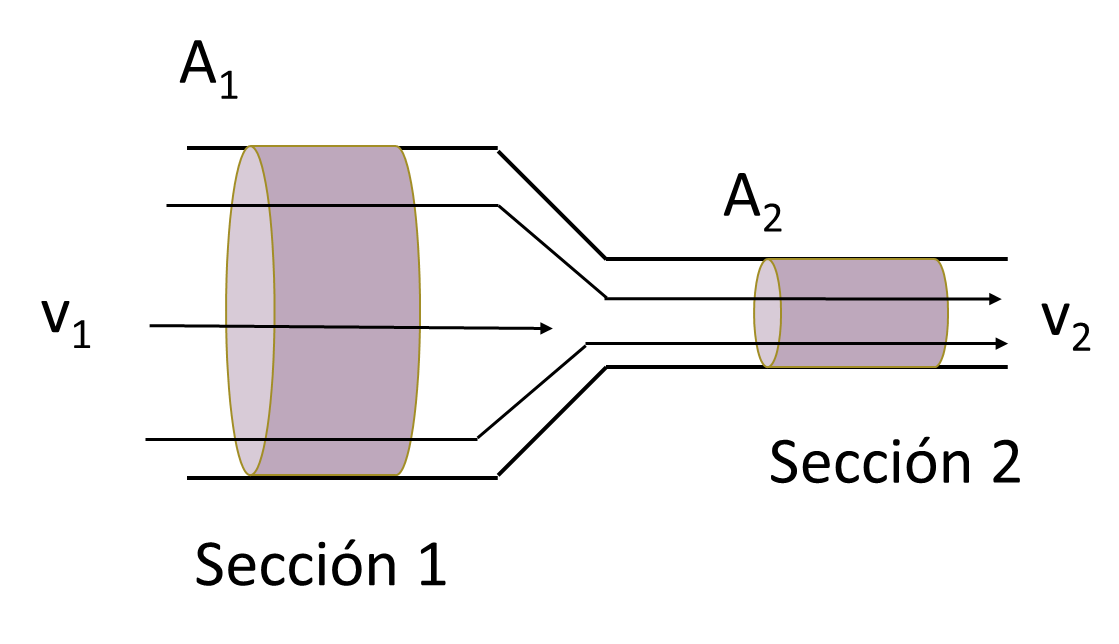
\includegraphics[scale=0.8]{Imagenes/Ejercicio_Bernoulli_01.png}
\end{figure}
\end{frame}
\begin{frame}
\frametitle{Ejercicio - Ec. de Bernoulli}
La velocidad en la sección 1 es de \SI[per-mode=symbol]{4}{\meter\per\second} a una presión de \SI{4d5}{\pascal}.
\\
\bigskip
\pause
¿Cuál es la velocidad y presión en la sección 2?
\end{frame}
\begin{frame}
\frametitle{Datos del enunciado}
\begin{minipage}{0.4\linewidth}
\begin{align*}
v_{2} &= ? \\[0.25em]
P_{2} &= ? \\[0.25em]
A_{1} &= \SI{0.02}{\square\meter} \\[0.25em]
A_{2} &= \SI{0.01}{\square\meter} \\[0.25em]
\end{align*}
\end{minipage}
\begin{minipage}{0.4\linewidth}
\begin{align*}
v_{1} &= \SI{4}{\meter\per\second} \\[0.25em]
P_{1} &= \SI{4d5}{\pascal}
\end{align*}
\end{minipage}
\end{frame}
\begin{frame}
\frametitle{Expresiones a utilizar}
Ecuación de continuidad:
\pause
\begin{eqnarray*}
\begin{aligned}
v_{1} \, A_{1} = v_{2} \, A_{2} \pause \hspace*{0.2cm} \Rightarrow \hspace*{0.2cm} v_{2} = \dfrac{v_{1} \, A_{1}}{a_{2}}
\end{aligned}
\end{eqnarray*}
\pause
Ecuación de Bernoulli:
\pause
\begin{align*}
P_{1} + \rho \, g \, h_{1} + \dfrac{1}{2} \rho \, v_{1}^{2} = P_{2} + \rho \, g \, h_{2} + \dfrac{1}{2} \rho \, v_{2}^{2}
\end{align*}
\end{frame}
\begin{frame}
\frametitle{Sustituciones}
Ecuación de continuidad:
\pause
\begin{eqnarray*}
\begin{aligned}
v_{2} &= \dfrac{\left(\SI[per-mode=fraction]{4}{\meter\per\second}\right) \left( \SI{0.02}{\square\meter}\right)}{\SI{0.01}{\square\meter}} = \\[0.5em] \pause
v_{2} &= \dfrac{\SI{0.08}{\square\meter} \unit[per-mode=fraction]{\meter\per\second}}{\SI{0.01}{\square\meter}} =  \\[0.5em] \pause
v_{2} &= \SI[per-mode=fraction]{8}{\meter\per\second}
\end{aligned}
\end{eqnarray*}
\end{frame}
\begin{frame}
\frametitle{Sustituciones}
Ecuación de Bernoulli, \pause En este ejercicio consideramos que las alturas $h_{1}$ y $h_{2}$, son iguales, es decir $h_{1} = h_{2} = h$.
\pause
\begin{eqnarray*}
\begin{aligned}
&P_{1} + \rho \, g \, h + \dfrac{1}{2} \rho \, v_{1}^{2} = P_{2} + \rho \, g \, h + \dfrac{1}{2} \rho \, v_{2}^{2} \\[0.5em] \pause
&P_{1} + \rho \, g \, (h - h) + \dfrac{1}{2} \rho \, v_{1}^{2} = P_{2} + \dfrac{1}{2} \rho \, v_{2}^{2} \\[0.5em] \pause
&P_{1} + \dfrac{1}{2} \rho \, v_{1}^{2} = P_{2} + \dfrac{1}{2} \rho \, v_{2}^{2}
\end{aligned}
\end{eqnarray*}
\end{frame}
\begin{frame}
\frametitle{Sustituciones}
\begin{eqnarray*}
\begin{aligned}    
&P_{2} - P_{1} = \dfrac{1}{2} \rho \, v_{1}^{2} - \dfrac{1}{2} \rho \, v_{2}^{2} \\[0.5em] \pause
&P_{2} - P_{1} = \dfrac{1}{2} \rho \, \left( v_{1}^{2} - v_{2}^{2} \right) \\[0.5em] \pause
&P_{2} = \dfrac{1}{2} \rho \, \left( v_{1}^{2} - v_{2}^{2} \right) + P_{1}
\end{aligned}
\end{eqnarray*}
\end{frame}
\begin{frame}
\frametitle{Sustituyendo los valores}
\begin{eqnarray*}
\begin{aligned}
P_{2} &= \dfrac{1}{2} \rho \, \left( v_{1}^{2} - v_{2}^{2} \right) + P_{1} = \\[0.5em] \pause
P_{2} &= \dfrac{1}{2} \left( \SI[per-mode=fraction]{d3}{\kilo\gram\per\cubic\meter} \right) \, \left[ \left( \SI[per-mode=fraction]{4}{\meter\per\second} \right)^{2} - \left( \SI[per-mode=fraction]{8}{\meter\per\second} \right)^{2} \right] + \SI{4d5}{\pascal} =  \\[0.5em] \pause
P_{2} &= - \SI{2.4d4}{\pascal} + \SI{4d5}{\pascal} =  \\[0.5em] \pause
P_{2} &= \SI{3.76d5}{\pascal}
\end{aligned}
\end{eqnarray*}
\end{frame}

\subsection{Casos especiales}

\begin{frame}
\frametitle{Revisión particular}
De acuerdo con el teorema de Bernoulli, se pueden presentar los siguientes casos:
\setbeamercolor{item projected}{bg=ao,fg=bananayellow}
\setbeamertemplate{enumerate items}{%
\usebeamercolor[bg]{item projected}%
\raisebox{1.5pt}{\colorbox{bg}{\color{fg}\footnotesize\insertenumlabel}}%
}
\begin{enumerate}[<+->]
\item Para un líquido estacionario.
\item Para una presión constante.
\item Para alturas iguales.
\end{enumerate}
\end{frame}
\begin{frame}
\frametitle{Para un líquido estacionario}
La velocidad de entrada y salida vale cero: $v_{1} = v_{2} = 0$:
\pause
\begin{eqnarray*}
\begin{aligned}
&P_{1} + \rho \, g \, h_{1} + \dfrac{1}{2} \rho \, v_{1}^{2} = P_{2} + \rho \, g \, h_{2} + \dfrac{1}{2} \rho \, v_{2}^{2} \\[0.5em] \pause
&P_{2} - P_{1} = \rho \, g \left( h_{2} - h_{1} \right)
\end{aligned}
\end{eqnarray*}
\end{frame}
\begin{frame}
\frametitle{Para una presión constante}
En este caso, se tiene que: $P_{1} = P_{2}$:
\pause
\begin{align*}
v = \sqrt{2 \, g \, h}
\end{align*}
La ecuación anterior fue desarrollada por el físico italiano Evangelista Torricelli (1608-1647).
\end{frame}
\begin{frame}
\frametitle{Teorema de Torricelli}
Quien enunció el siguiente teorema que lleva su nombre: \pause la magnitud de la velocidad con que sale un líquido por el orificio de un recipiente es igual a la que adquiere un objeto que se deje caer libremente desde la superficie libre del líquido hasta el nivel del orificio.
\end{frame}
\begin{frame}
\frametitle{Para alturas iguales}
En este caso, se tiene que $h_{1} = h_{2}$:
\pause
\begin{align*}
P_{1} + \rho \, g + \dfrac{1}{2} \rho \, v_{1}^{2} = P_{2} + \rho \, g + \dfrac{1}{2} \rho \, v_{2}^{2}
\end{align*}
\end{frame}

\subsection{Teorema de Torricelli}

\begin{frame}
\frametitle{Aplicación del principio de Bernoulli}
Una aplicación del principio de Bernoulli es cuando se desea conocer la velocidad de salida de un líquido a través de un orificio de un recipiente.
\end{frame}
\begin{frame}
\frametitle{Puntos relevantes}    
Considerando que es un recipiente muy grande y abierto, además haciendo las consideraciones siguientes:
\setbeamercolor{item projected}{bg=black,fg=white}
\setbeamertemplate{enumerate items}{%
\usebeamercolor[bg]{item projected}%
\raisebox{1.5pt}{\colorbox{bg}{\color{fg}\footnotesize\insertenumlabel}}%
}
\begin{enumerate}[<+->]
\item La presión en la superficie libre del líquido es igual a la presión atmosférica.
\seti
\end{enumerate}
\end{frame}
\begin{frame}
\frametitle{Puntos relevantes}    
\setbeamercolor{item projected}{bg=black,fg=white}
\setbeamertemplate{enumerate items}{%
\usebeamercolor[bg]{item projected}%
\raisebox{1.5pt}{\colorbox{bg}{\color{fg}\footnotesize\insertenumlabel}}%
}
\begin{enumerate}[<+->]    
\conti
\item La velocidad es despreciable si la comparamos con la salida del líquido por el orificio, por lo que se puede eliminar la energía cinética de la ecuación de Bernoulli en este punto.
\seti
\end{enumerate}
\end{frame}
\begin{frame}
\frametitle{Puntos relevantes}    
\setbeamercolor{item projected}{bg=black,fg=white}
\setbeamertemplate{enumerate items}{%
\usebeamercolor[bg]{item projected}%
\raisebox{1.5pt}{\colorbox{bg}{\color{fg}\footnotesize\insertenumlabel}}%
}
\begin{enumerate}[<+->]    
\conti
\item La profundidad, es decir, $h$, es la distancia que hay desde la superficie sobre el líquido hasta el orificio.
\item En el orificio, la altura es $h = 0$, y la presión es igual a la atmosférica.
\end{enumerate}
\end{frame}
\begin{frame}
\frametitle{Esquema para el teorema de Torricelli}
\begin{figure}
    \centering
    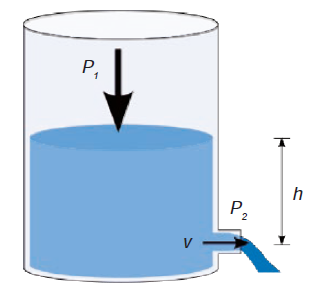
\includegraphics[scale=0.75]{Imagenes/Ejercicio_Torricelli.png}
\end{figure}
\end{frame}
\begin{frame}
\frametitle{Con la ecuación de Bernoulli}
Si consideramos que el subíndice $1$ pertenece a todos los datos correspondientes al orifico de entrada y el subíndice $2$ a todo lo relativo al orificio de salida:
\pause
\begin{align*}
P_{1} + \rho \, g \, h_{1} + \dfrac{1}{2} \rho \, v_{1}^{2} = P_{2} + \rho \, g \, h_{2} + \dfrac{1}{2} \rho \, v_{2}^{2}
\end{align*}    
\end{frame}
\begin{frame}
\frametitle{Revisando las variables}
Se tiene entonces que:
\pause
\begin{eqnarray*}
\begin{aligned}
&h_{1} = 0, \pause \hspace*{0.4cm} h_{2} = h, \pause \hspace*{0.4cm} P_{1} = P_{2} = P, \pause \hspace*{0.4cm} v_{2} = 0 \\[0.5em] \pause
&P + \dfrac{1}{2} \rho \, v_{1}^{2} = P + \rho \, g \, h_{2} \\[0.5em] \pause
&\dfrac{1}{2} \rho \, v_{1}^{2} = \rho \, g \, h_{2} \pause \hspace{1.5cm} \dfrac{1}{2} \rho \, v_{1}^{2} = \rho \, g \, h \\[0.5em] \pause
&v = \sqrt{ 2 \, g \, h}
\end{aligned}
\end{eqnarray*}
\end{frame}
\begin{frame}
\frametitle{Teorema de Torricelli}
La velocidad con que sale el agua por un orificio es la misma que hubiera adquirido en caída libre desde una altura $h_{1} - h_{2}$.
\end{frame}
\begin{frame}
\frametitle{Ejercicio - Teorema Torricelli}
Un tanque abierto tiene un orificio de \SI{1.5}{\centi\meter} de radio, el cual se encuentra a \SI{3}{\meter} por debajo del nivel del agua contenida en el tanque.
\\
\bigskip
\pause
¿Cuál es la velocidad con que sale el agua?
\end{frame}
\begin{frame}
\frametitle{Solución al Ejercicio}
Datos del enunciado:
\pause
\begin{align*}
h &= \SI{3}{\meter} \\[0.5em]
g &= \SI[per-mode=fraction]{9.81}{\meter\per\square\second}
\end{align*}
\end{frame}
\begin{frame}
\frametitle{Expresión y sustitución}
La expresión es:
\pause
\begin{align*}
v = \sqrt{ 2 \, g \, h}
\end{align*}
\pause
Sustituyendo los valores:
\pause
\begin{eqnarray*}
\begin{aligned}
v &= \sqrt{2 \left( \SI[per-mode=fraction]{9.81}{\meter\per\square\second} \right)\left( \SI{3}{\meter}  \right)} = \pause \SI[per-mode=fraction]{7.67}{\meter\per\second}
\end{aligned}
\end{eqnarray*}
\end{frame}
\begin{frame}
\frametitle{Ejercicio}
Determinar la profundidad a la que se debe encontrar un orificio en un tanque de almacenamiento, para que por éste salga un líquido a una velocidad de \SI[per-mode=symbol]{4.5}{\meter\per\second}
\end{frame}
\begin{frame}
\frametitle{Datos del enunciado}
\begin{align*}
h &= ? \\[0.5em]
v &= \SI[per-mode=symbol]{4.5}{\meter\per\second} \\[0.5em]
g &= \SI[per-mode=symbol]{9.8}{\meter\per\square\second}
\end{align*}
\end{frame}
\begin{frame}
\frametitle{Expresión y sustitución}
Ocupamos la expresión:
\pause
\begin{eqnarray*}
\begin{aligned}
v = \sqrt{2 \, g \, h} \pause \hspace*{0.3cm} \Rightarrow \hspace*{0.3cm} h = \dfrac{v^{2}}{2 \, g}
\end{aligned}
\end{eqnarray*}
Sustituimos los valores:
\pause
\begin{eqnarray*}
\begin{aligned}
h &= \dfrac{v^{2}}{2 \, g} = \dfrac{\left( \SI[per-mode=symbol]{4.5}{\meter\per\second} \right)^{2}}{ 2 \left( \SI[per-mode=symbol]{9.8}{\meter\per\square\second}\right)} = \\[0.5em] \pause
h &= \dfrac{\SI[per-mode=symbol]{20.25}{\square\meter\per\square\second}}{\SI[per-mode=symbol]{19.62}{\meter\per\square\second}} = \pause \SI{1.032}{\meter}
\end{aligned}
\end{eqnarray*}
\end{frame}
\begin{frame}
\frametitle{Ejercicio}
Por una tubería de \SI{5.08}{\centi\meter} de diámetro circula agua a una magnitud de velocidad de \SI[per-mode=symbol]{1.6}{\meter\per\second}.
\\
\bigskip
\pause
Calcula la magnitud de velocidad que llevará el agua al pasar por un estrechamiento de la tubería donde el diámetro es de \SI{4}{\centi\meter}.
\end{frame}
\begin{frame}
\frametitle{Datos del enunciado}
\begin{align*}
d_{1} &= \SI{5.08}{\centi\meter} \\[0.5em]
d_{2} &= \SI{4}{\centi\meter} \\[0.5em]
v_{1} &= \SI[per-mode=symbol]{1.6}{\meter\per\second} \\[0.5em]
v_{2} &= ?
\end{align*}
\end{frame}
\begin{frame}
\frametitle{Expresiones y sustitución}
Vamos a requerir la expresión para obtener el área de un círculo:
\pause
\begin{align*}
A = \pi \, \dfrac{d^{2}}{4}
\end{align*}
\pause
La ecuación de continuidad:
\pause
\begin{eqnarray*}
\begin{aligned}
v_{1} \, A_{1} = v_{2} \, A_{2} \pause \hspace*{0.3cm} \Rightarrow \hspace*{0.3cm} v_{2} = \dfrac{v_{1} \, A_{1}}{A_{2}}
\end{aligned}
\end{eqnarray*}
\end{frame}
\begin{frame}
\frametitle{Calculando las secciones transversales}
Para el área con el diámetro mayor:
\pause
\begin{eqnarray*}
\begin{aligned}
A_{1} = \dfrac{\pi (\SI{5.08}{\centi\meter})^{2}}{4} = \pause \SI{20.26}{\square\centi\meter}
\end{aligned}
\end{eqnarray*}
\pause
Para el área con el diámetro menor:
\pause
\begin{eqnarray*}
\begin{aligned}
A_{2} = \dfrac{\pi (\SI{4}{\centi\meter})^{2}}{4} = \pause \SI{12.56}{\square\centi\meter}
\end{aligned}
\end{eqnarray*}
\end{frame}
\begin{frame}
\frametitle{Calculando la velocidad}
Se tiene entonces que la velocidad $v_{2}$ es:
\pause
\begin{eqnarray*}
\begin{aligned}
v_{2} &= \dfrac{\left( \SI{20.26}{\square\centi\meter}\right) \left( \SI[per-mode=symbol]{1.6}{\meter\per\second}\right)}{\SI{12.56}{\square\centi\meter}} = \\[0.5em] \pause
v_{2} &= \SI[per-mode=symbol]{2.58}{\meter\per\second}
\end{aligned}
\end{eqnarray*}
\end{frame}

\section{Calor y temperatura}
\frame{\tableofcontents[currentsection, hideothersubsections]}
\subsection{Actividad de desarrollo}

\begin{frame}
\frametitle{Trabajo a realizar}
Para acompañar el desarrollo del tema de \textocolor{red}{calor} y \textocolor{ao}{temperatura}, se te pide que investigues lo siguiente:
\end{frame}
\begin{frame}
\frametitle{Puntos a desarrollar}
\setbeamercolor{item projected}{bg=cerulean,fg=black}
\setbeamertemplate{enumerate items}{%
\usebeamercolor[bg]{item projected}%
\raisebox{1.5pt}{\colorbox{bg}{\color{fg}\footnotesize\insertenumlabel}}%
}
\begin{enumerate}[<+->]
\item Un breve biografía de Anders Celsius, Gabriel Daniel Fahrenheit y William Thompson.
\item Describir la manera en que se construyeron las escalas de temperatura: Celsius, Fahrenheit y Kelvin.
\item Determinar de manera analítica el punto en el que las escalas Celsius y Fahrenheit tienen el mismo valor.
\end{enumerate}
\end{frame}
\begin{frame}
\frametitle{Evaluación del Trabajo}
Esta actividad otorgará hasta $6$ puntos en Evaluación Continua.
\\
\bigskip
\pause
La calidad del trabajo será claramente de mayor reto para lograr el puntaje máximo.
\end{frame}
\begin{frame}
\frametitle{Evaluación del Trabajo}
Se indicará la rúbrica de evaluación para el trabajo, se pide gentilmente la consulta de libros, revistas, sitios de internet, haciendo la correspondiente referencia en formato APA.
\\
\bigskip
\pause
Actividad que se entregue ocupando sitios como ChatGPT, etc. no serán evaluados a pesar de enviarse.
\end{frame}
\begin{frame}
\frametitle{Fecha de entrega}
Se abrirá asignación en Teams para enviar el documento, teniendo como fecha límite el martes 4 de julio a las 8 pm.
\\
\bigskip
\pause
El desarrollo del trabajo y envío del mismo es INDIVIDUAL.
\end{frame}
\begin{frame}
\frametitle{Fecha de entrega}
No se recibirán trabajos de manera extemporánea, a menos que se tenga la evidencia de problemas técnicos al momento del envío, debiendo notificar a la Coordinación Académica y al Profesor, \pause así se les solicitará en mensaje directo el envío de su actividad.
\end{frame}

\section{Práctica 5}
\frame{\tableofcontents[currentsection, hideothersubsections]}
\subsection{Trabajo previo}

\begin{frame}
\frametitle{Preparando la Práctica}
En la siguiente clase de Laboratorio, se trabajará la \textocolor{carmine}{Práctica 5. Medición de la temperatura}.
\\
\bigskip
\pause
Se considerará parte de la evaluación en: \textocolor{red}{Preparación} y \textocolor{ao}{Participación}. En caso de no traer el trabajo previo, la calificación en la rúbrica será de $0$ puntos.
\end{frame}

\end{document}